% Part of the layout information as well as title, logo are defined in the style file, e.g. beamerthemeOregon.sty
\documentclass{beamer}
\mode<presentation>
{
  \usetheme{NCAR}
  \setbeamercovered{transparent}
}
\usepackage{times}


\usepackage{amsmath,amssymb}
\usepackage[english]{babel}
\usepackage[latin1]{inputenc}
\usepackage[orientation=landscape,size=a0,scale=1,debug]{beamerposter}   % scale only seems to apply to text
\usepackage{framed, color} % to produce boxes, e.g. for conclusions
\definecolor{shadecolor}{RGB}{169,202,222}

\usepackage{ragged2e} % to use \justifying

\usepackage{natbib}
 \def\newblock{\hskip .11em plus .33em minus .07em}

\usepackage[absolute,overlay]{textpos}
\TPGrid[0cm,0cm]{100}{100} % choose \TPHorizModule and \TPVertModule so as to give a grid of 100 intervals across and 100 intervals down
\TPMargin{1cm}

\textblockorigin{0mm}{90mm} %sets the origin of the page - the 0,0 point of the coordinate system

\usepackage{tikz}
% \usetikzlibrary{snakes}

\title[]{{The Development of Quantitative Hydrologic Storylines to Understand Uncertainty in Climate}}

\makeatletter
\def\beamer@andinst{\\[0.1em]}
\makeatother

\author[]{Ethan Gutmann\inst{1}, \and Martyn Clark\inst{1}, \and Andy Wood\inst{1}, \and Joseph Hamman\inst{1}, \and Julie Vano\inst{1}, \and Levi Brekke\inst{1}, \and Ken Nowak\inst{2}, \and Jeffrey Arnold\inst{3}}
\institute[]{\inst{1}National Center for Atmospheric Research, Research Applications Lab, Boulder, United States \and \inst{2}Bureau of Reclamation, Denver, United States \and \inst{3}US Army Corps of Engineers, Climate Preparedness and Resilience Programs, United States}

\date{April 2017}

\newcommand{\degC}{$^{\circ}$C}

\setbeamertemplate{caption}{\insertcaptionname~\insertcaptionnumber:
\insertcaption}

\begin{document}

\begin{frame}{}
 \vspace{2cm}

 \begin{columns}

  %%% FIRST COLUMN

  \begin{column}{.3333\paperwidth} % if all columns have the same width, it's enough to declare that width once

   \begin{textblock}{\textwidth \TPHorizModule}(0,0)
    \begin{block}{1. Introduction}

     \begin{itemize}
      \justifying

      \item Future climate projections are inherently uncertain, and quantifying and managing this uncertainty is one of the key tasks in any climate application.
      \item Previous research assessing climate change impacts on hydrologic systems shows a need to understand the sources of this uncertainty so that future work can reduce uncertainty, and so that the most realistic assessment of uncertainty can be presented.
      \item This uncertainty stems from chaotic variability in the climate system \citep{Deser_2014} and from the uncertain nature of the methods we use \citep{Gutmann_2012,Mendoza_2016,Mizukami_2016,Clark_2016} (either from lack of understanding of the system or intentional simplifications in our models.)
      \item We focus on quantifying the uncertainty that comes from methodological choices related to emissions scenarios, climate models, downscaling methods, and hydrology models and parameters (see Figure \ref{fig:storylines}).

     \end{itemize}

    \end{block}
   \end{textblock}


   \begin{textblock}{\textwidth \TPHorizModule}(0,18)
    \begin{block}{2. Hydrologic Storylines}

     \begin{itemize}
      \justifying

      \item We aim to develop a set of representative hydrologic projections or ``storylines'' while specifically addressing the leading contributors of uncertainty.
      \item The first step is to characterize the uncertainties in the ``full'' ensemble in order to understand where and how much each component of the model chain contributes to the full ensemble's uncertainty.
      \item The second phase of the project will focus on reducing uncertainties by refining methodologies and eliminating unlikely ensemble members.
      \item Finally, distinct hydrologic storylines will be developed using data-driven and bottom-upsampling methods to represent the range of likely outcomes with a minimum number of ensemble members.

     \end{itemize}

     \begin{figure}
      \center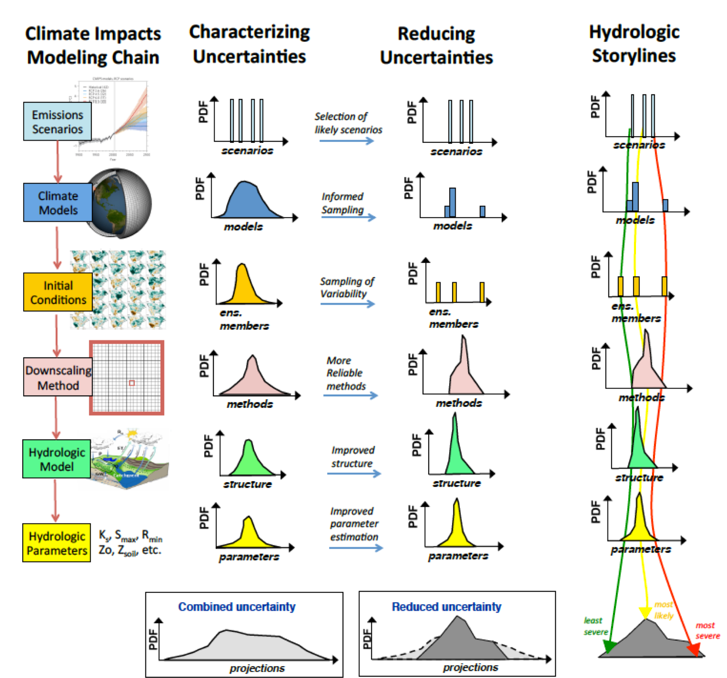
\includegraphics[width=\linewidth]{figures/storylines_diag.png}
      \caption{Schematic on approaches to explicitly characterize and reduce the myriad uncertainties in assessments of the hydrologic impacts of climate change and the development of representative quantitative hydrologic storylines for specific applications. Caption and figure from \citep{Clark_2016}.
       \label{fig:storylines}}
     \end{figure}

    \end{block}
   \end{textblock}


   %%% SECOND COLUMN

   \begin{textblock}{\textwidth \TPHorizModule}(33.333,0)
    \begin{block}{3. Downscaling}

     \begin{tikzpicture}[]

      % draw horizontal line
      \draw (0,0) -- (33.333,0);
      %   \draw[snake] (2,0) -- (4,0);
      %   \draw (4,0) -- (5,0);
      %   \draw[snake] (5,0) -- (7,0);

      % draw vertical lines
      \foreach \x in {0,5,12,22,33.333}
      \draw[->,line width=3pt] (\x cm,0) -- (1+\x cm,0);

      % draw nodes
      \draw (0,0) node[below=3pt] {Raw GCM};
      \draw (5,0) node[below=3pt] {BCSD};
      \draw (12,0) node[below=3pt] {Multivariate Regression};
      \draw (22,0) node[below=3pt] {Reduced Physics RCM};
      \draw (31,0) node[below=3pt] {High-res RCM};

      \node[above,font=\large\bfseries] at (current bounding box.north) {The complexity continuum of climate downscaling methodologies};

     \end{tikzpicture}

     \begin{itemize}
      \justifying

      \item Not all downscaling methods are created equal. Some methods create artifacts even in historical climate \citep{Gutmann_2014}, with implications for hydrologic modeling \citep{Mizukami_2016}. The sensitivity of the climate change signal to downscaling methodology has not been widely explored.
      \item We are developing the Generalized Analog Regression Downscaling (GARD) tool to provide a simple statistical downscaling method capable of implementing a variety of statistical transformations from various inputs (e.g. precipitation, humidity, wind, PCA, etc.) to various outputs (e.g. precipitation, temperature, etc.) See http://gard.readthedocs.io/.
      \item We have developed a quasi-dynamical downscaling tool ICAR, the Intermediate Complexity Atmospheric Research model \citep{Gutmann_2016} to provide a downscaling option in between a full physics RCM and a statistically based tool.
      \item Simple / existing downscaling methods (e.g. BCSD) are being compared to progressively more complex methods like GARD, ICAR, and WRF to better understand how methodological complexity is related to fidelity and sensitivity.

     \end{itemize}

     \vspace{-0.5cm}
     \begin{figure}
      \center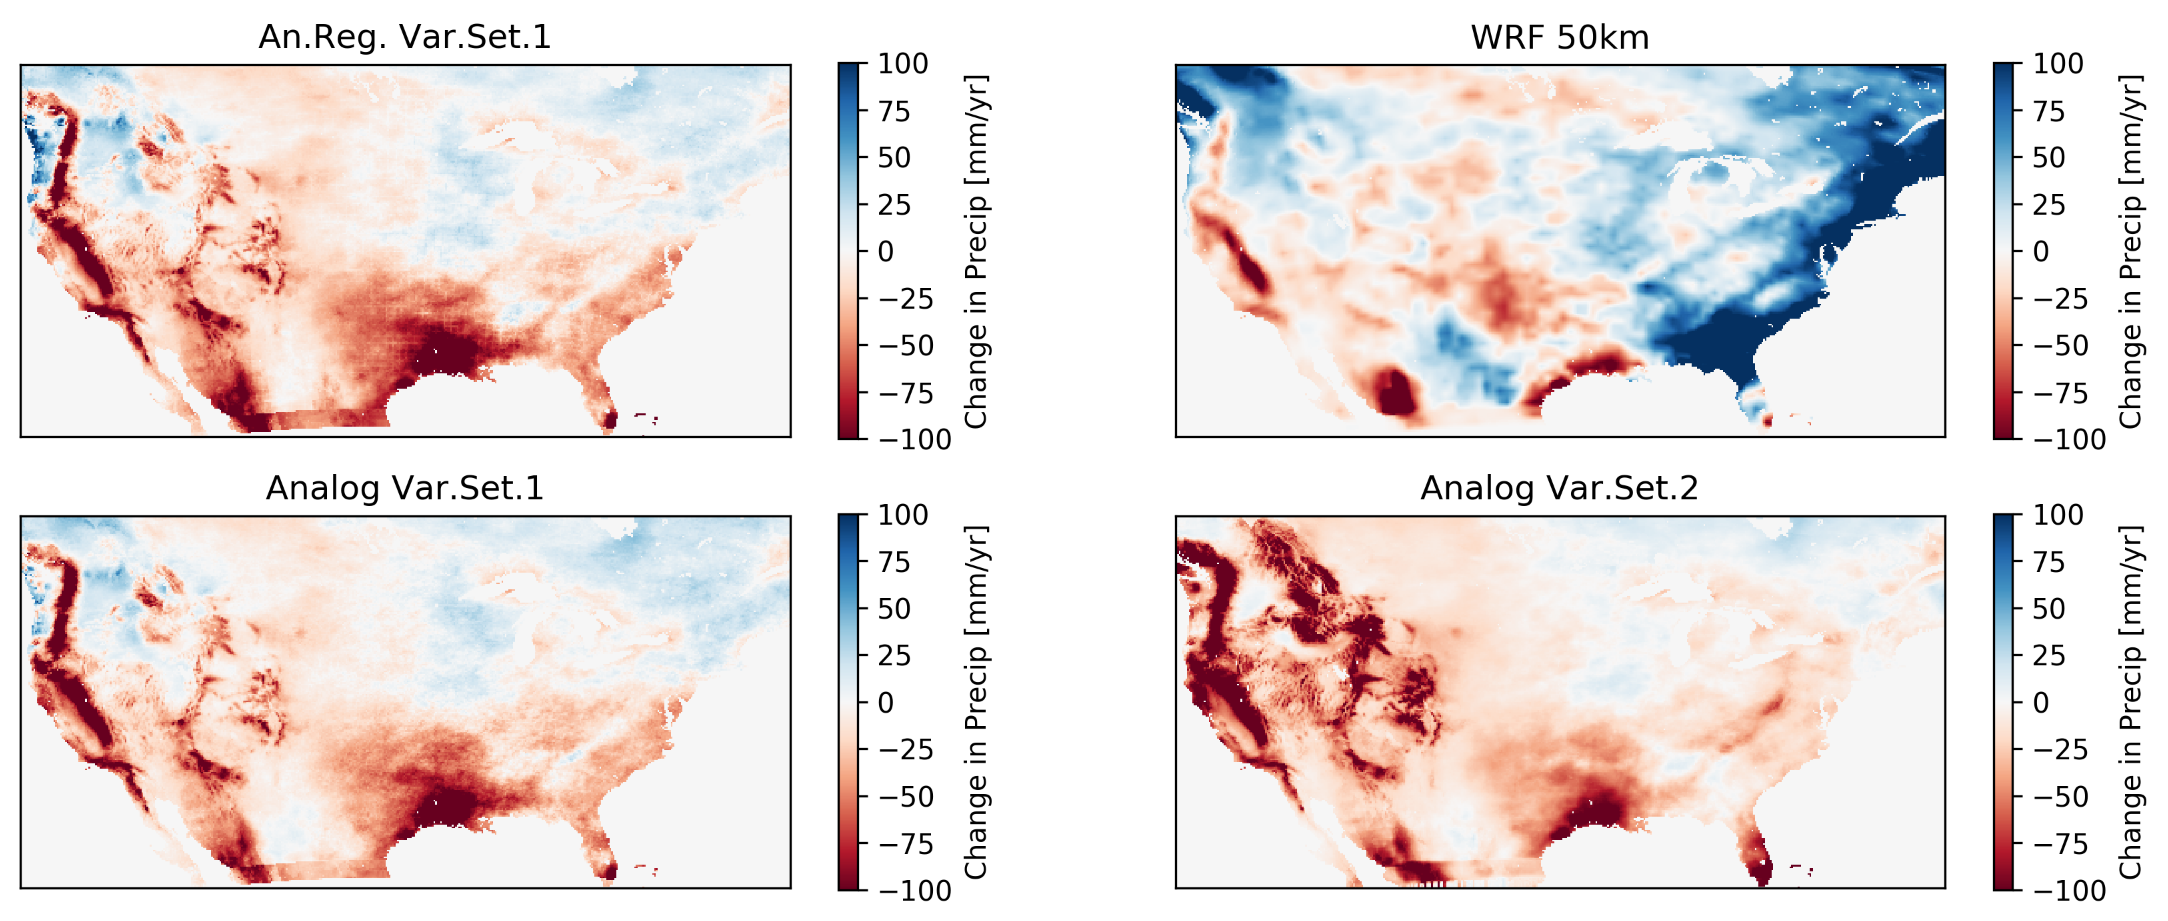
\includegraphics[width=0.85\linewidth]{figures/deltas.png}
      \caption{Changes in precipitation over CONUS from 4 downscaling approaches applied to an RCM. Top-left analog-regression scheme precipitation as input, top-right the raw 50km RCM, bottom-left: analog scheme precipitation as input, bottom-right: analog scheme applied to a combination of precipitation and upper-air circulation.}
      \label{fig:downscaling}
     \end{figure}

    \end{block}

   \end{textblock}



   \begin{textblock}{\textwidth \TPHorizModule}(33.333,45)
    \begin{block}{4. Hydrologic Modeling}

        \begin{itemize}
         \justifying
         \item Typical hydrologic climate impacts studies do not explore how hydrologic model structure or model parameters influence the inferences derived from the modeling activity.
         \item We will compare climate signals from traditional models such as VIC, and an ensemble of different modeling approaches using the new multi-physics Structure for Unifying Multiple Modeling Alternatives (SUMMA) model \citep{Clark_2015} (see Figure \ref{fig:summa}). Using SUMMA allows for the controlled and systematic analysis of modeling options and complexities.
         \item In addition, an ensemble of model parameters will be tested, including parameters derived using the Multi-scale Parameter Regionalization (MPR) method of \citet{Samaniego_2010}. Using MPR allows for the generation of ensembles of parameters, derived from calibrations performed using an array of objective functions.
        \end{itemize}

     \begin{figure}
      \center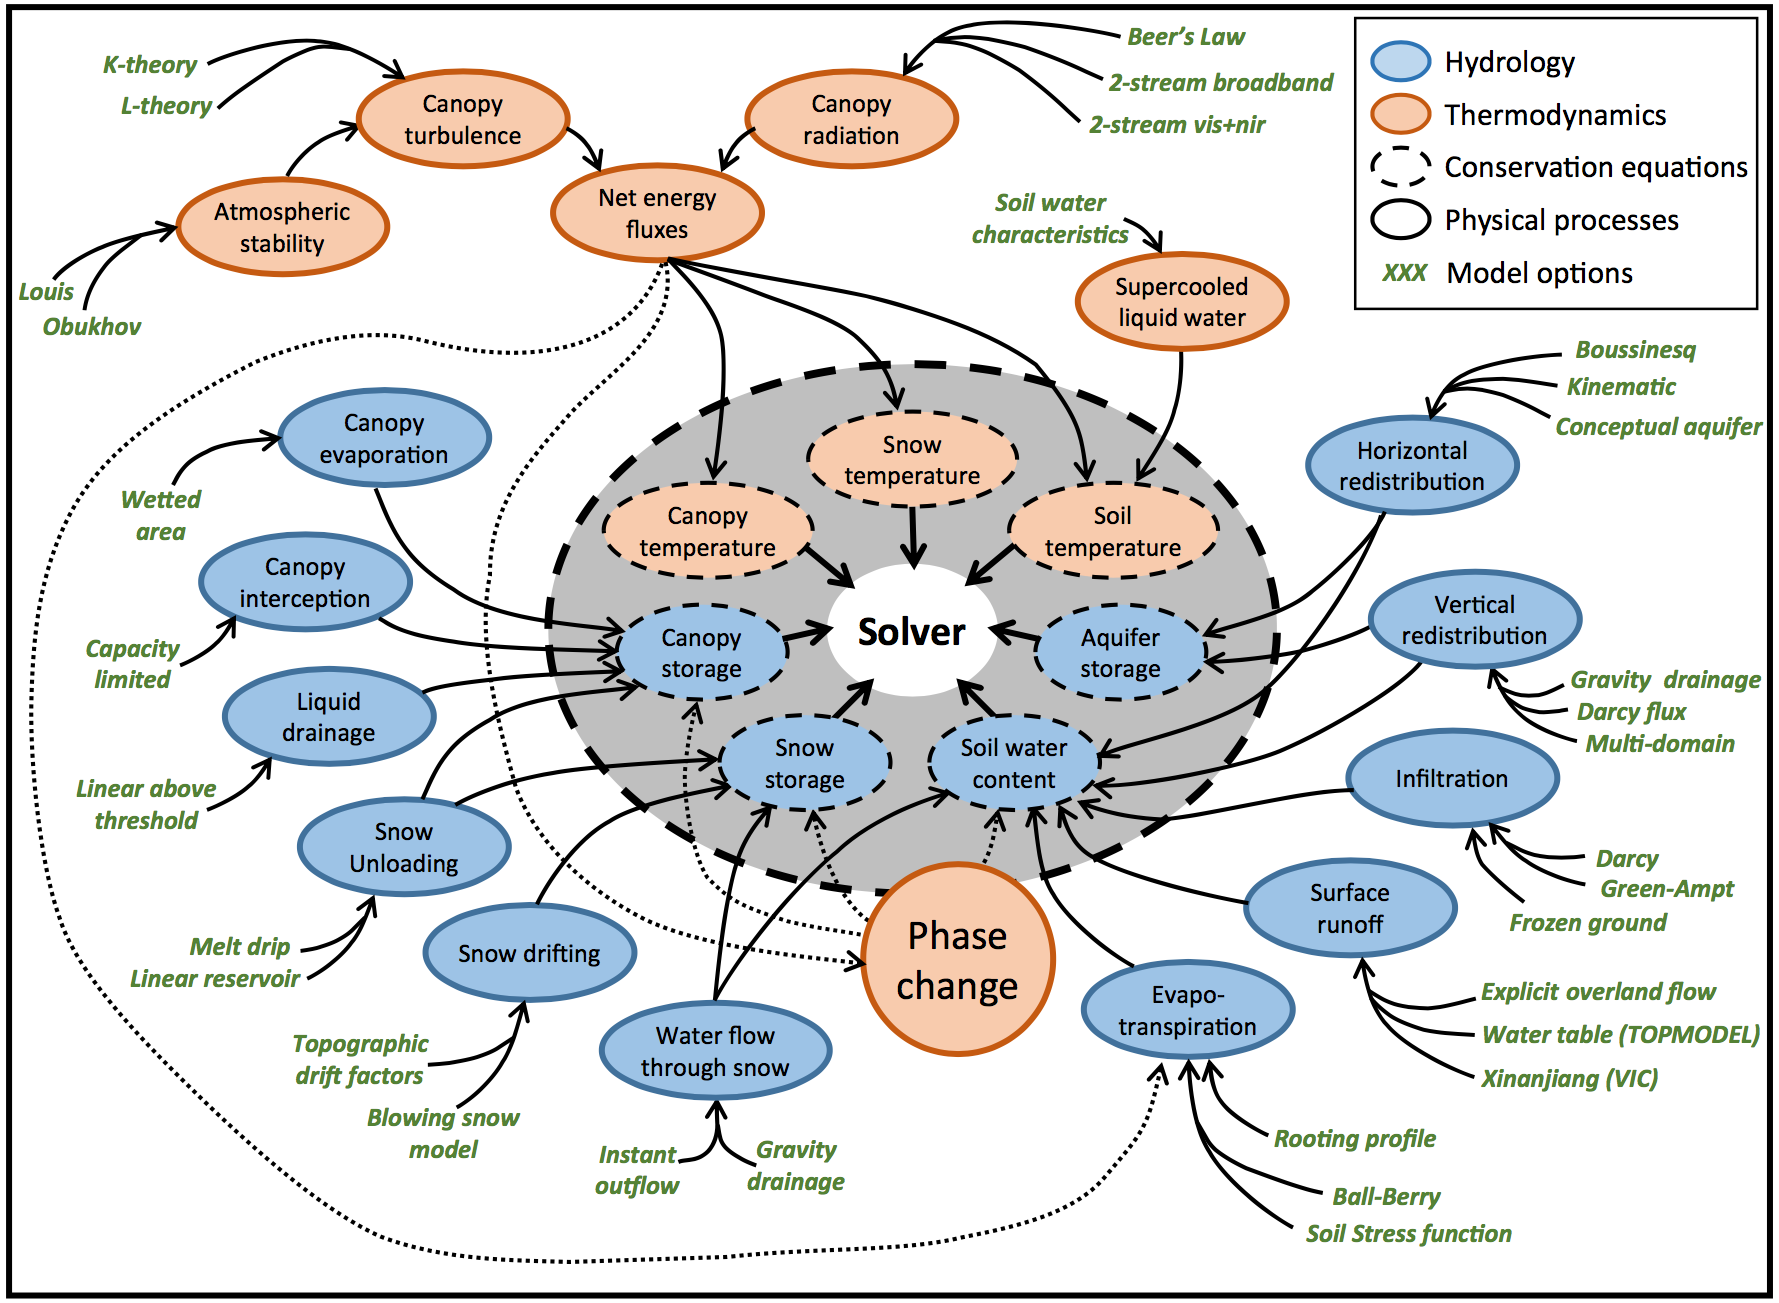
\includegraphics[width=0.6\linewidth]{figures/summa.png}
      \caption{The SUMMA framework for supporting multiple alternative model options for a range of physical processes, integrated with a common numerical solver. Figure from \citet{Clark_2015}.}
      \label{fig:summa}
     \end{figure}

    \end{block}
   \end{textblock}


   %%% THIRD COLUMN

   \begin{textblock}{\textwidth \TPHorizModule}(66.667,0)
    \begin{block}{5. Outlook: Production of large ensembles of hydrologic projections}

     \begin{itemize}
      \justifying
      \item We are developing a large ensemble of hydrologic projections over the CONUS domain.
      \item Our controlled evaluation of both the climate forcing and hydrologic modeling will allow for increased understanding of uncertainty derived from each component of the climate impacts modeling chain.
     \end{itemize}

     \begin{figure}
      \center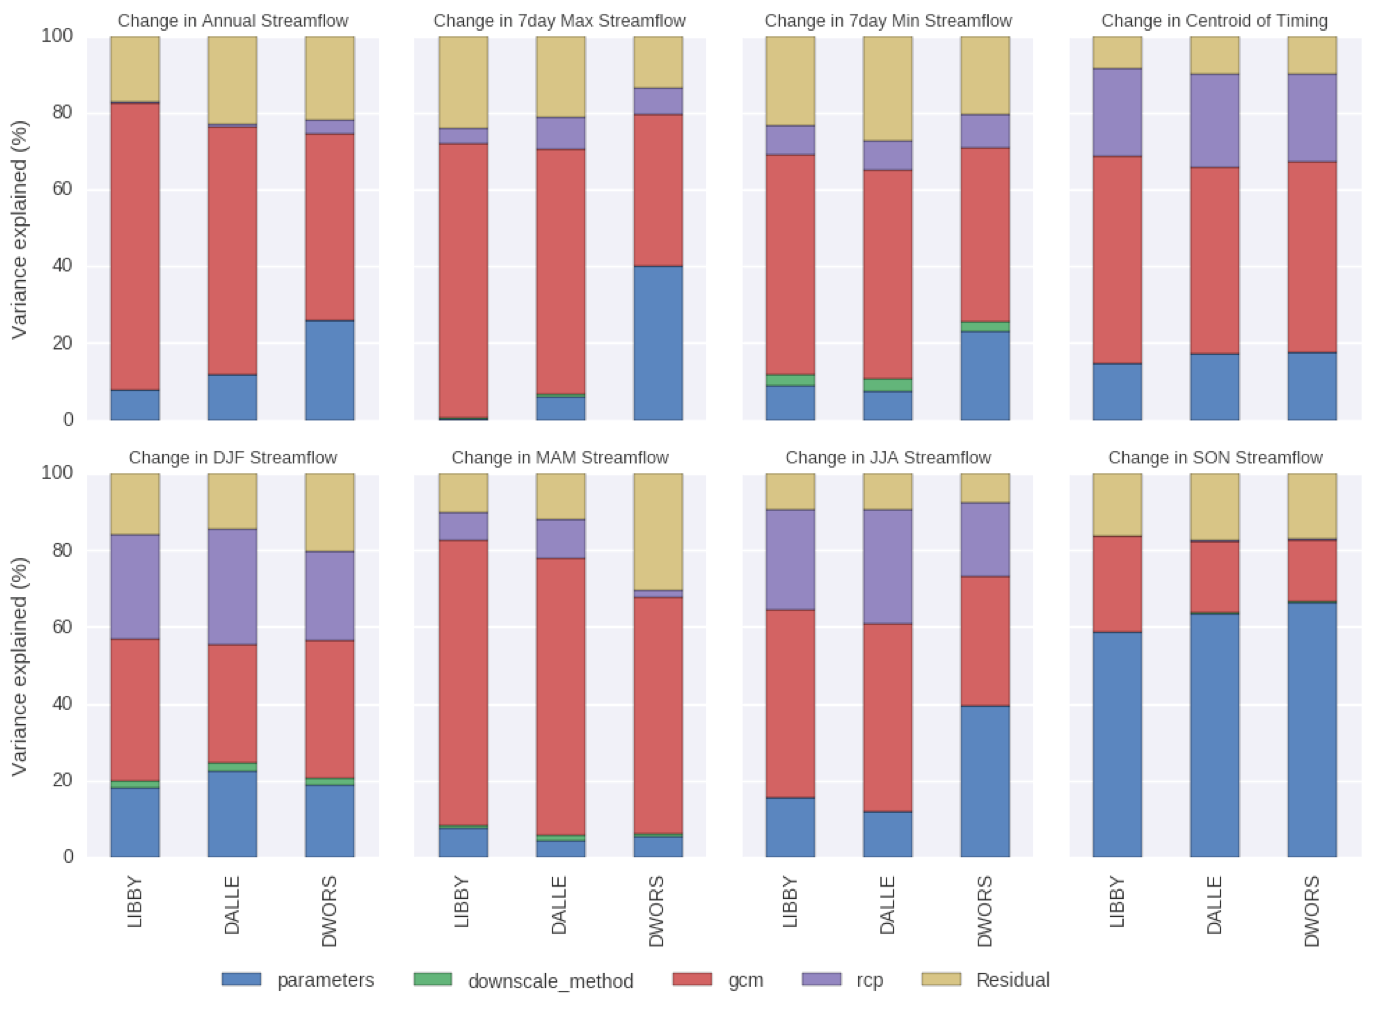
\includegraphics[width=0.75\linewidth]{figures/anova.png}
      \caption{Example of an ANOVA analysis performed using a combination of existing data from the University of Washington RMJOC dataset and the NCAR BCSD dataset. The total dataset includes 2 RCPs, 31 GCMs, 2 simple downscaling methods, 1 hydrologic model (VIC), and 4 hydrologic model parameter sets. Each subplot represents a different analysis metric. Each column is a different watershed in the Columbia River Basin.
       \label{fig:anova}}
     \end{figure}

     \begin{itemize}
      \justifying
      \item Figure \ref{fig:anova} provides an example, using existing datasets, of how uncertainty (variance) can be partitioned.
      \item Key point: the variance explained by each variable is differs between analysis metrics.
     \end{itemize}

    \end{block}
   \end{textblock}

   \begin{textblock}{\textwidth \TPHorizModule}(66.667,45)


    \begin{block}{6. Conclusions}

     \vspace{-1cm}
     \begin{shaded}
      \begin{itemize}         \vspace{1cm}
       \justifying
       \item Hydrologic climate projections have uncertainty from the climate forcing (emissions scenarios, climate models, initial conditions) and from the hydrologic modeling application (model structure and parameters). We are systematically characterizing these uncertainties. \vspace{1cm}
       \item We are developing new climate downscaling tools (e.g. GARD, ICAR) to fill in the complexity continuum. These tools will facilitate the generation of large ensembles of climate forcings and new analysis approaches that target the relationship between model diversity, fidelity, and sensitivity. \vspace{1cm}
       \item New data-driven and bottom-up sampling methods are being developed to enable the selection of smaller sets of representative hydrologic projections (storylines) while addressing the leading contributors of uncertainty. \vspace{1cm}

      \end{itemize}

     \end{shaded}
     \vspace{-1cm}

    \end{block}
   \end{textblock}

   \begin{textblock}{\textwidth \TPHorizModule}(66.667,69)
   \vspace{-2cm}
    \begin{block}{References}


     \justifying
     \bibliographystyle{apalike}

     \scriptsize\bibliography{library} % this command does not accept white spaces in the path

    \end{block}
   \end{textblock}


  \end{column}
 \end{columns}
\end{frame}

\end{document}
